\documentclass{article}[12pt]
\usepackage{color}
\usepackage[normalem]{ulem}
\usepackage{times}
\usepackage{listings}
\usepackage{fullpage}
\usepackage{amsmath}
\usepackage{amssymb}
\usepackage{tikz}
\def \R {\mathbb R}
\def \imp {\Longrightarrow}
\def \eps {\varepsilon}
\def \Inf {{\sf Inf}}
\newenvironment{proof}{{\bf Proof.  }}{\hfill$\Box$}
\newtheorem{theorem}{Theorem}[section]
\newtheorem{definition}{Definition}[section]
\newtheorem{corollary}{Corollary}[section]
\newtheorem{lemma}{Lemma}[section]
\newtheorem{claim}{Claim}[section]
\setlength {\parskip}{2pt}
\setlength{\parindent}{0pt}

\newcommand{\headings}[4]{\noindent {\bf Assignment 15 CME241} \hfill {{\bf Author:} Nicolas Sanchez} \\
{} \hfill {{\bf Due Date:} #2} \\

\rule[0.1in]{\textwidth}{0.025in}
}

\newcommand{\klnote}[1]{{\color{red} #1}}
\newcommand{\klsout}[1]{{\color{red} \sout{#1}}}

\begin{document}

\headings{\#1}{Tuesday, October 8, 10:30am}\section{} 



\section{Implementation of functions}
We implement the described functions in the given file and include them here:
\begin{lstlisting}
def get_mc_value_function(
    state_return_samples: Sequence[Tuple[S, float]]
) -> ValueFunc:
    """
    Implement tabular MC Value Function compatible with the interface defined above.
    """
    sum_tracker = {}
    count_tracker = {}
    value_tracker ={}
    for s,returns_ in state_return_samples:
        sum_tracker[s] = sum_tracker.get(s,0.)+returns_
        count_tracker[s] = count_tracker.get(s,0)+1
        value_tracker[s] = sum_tracker[s]/float(count_tracker[s])
    return value_tracker
  
def get_probability_and_reward_functions(
    srs_samples: Sequence[Tuple[S, float, S]]
) -> Tuple[ProbFunc, RewardFunc]:
    """
    Implement code that produces the probability transitions and the
    reward function compatible with the interface defined above.
    """
    prob_tracker = {}
    reward_tracker = {}
    count_tracker = {}
    for s1,r,s2 in srs_samples:
        reward_tracker[s1] = reward_tracker.get(s1,0.) + r
        prob_tracker[s1] = prob_tracker.get(s1,{})
        prob_tracker[s1][s2] = prob_tracker[s1].get(s2,0) + 1
        count_tracker[s1] = count_tracker.get(s1,0) + 1

    for s_from in prob_tracker:
        reward_tracker[s_from] = reward_tracker[s_from]/float(count_tracker[s_from])
        for s_to in prob_tracker[s_from]:
            prob_tracker[s_from][s_to] = float(prob_tracker[s_from][s_to])/float(count_tracker[s_from])

    return prob_tracker, reward_tracker

def get_mrp_value_function(
    prob_func: ProbFunc,
    reward_func: RewardFunc
) -> ValueFunc:
    """
    Implement code that calculates the MRP Value Function from the probability
    transitions and reward function, compatible with the interface defined above.
    Hint: Use the MRP Bellman Equation and simple linear algebra
    """
    states_set = reward_func.keys()
    num_states = len(states_set)
    prob_matrix = np.zeros((num_states,num_states))
    rew_vector = np.zeros((num_states))
    
    for i, s1 in enumerate(states_set):
        rew_vector[i] = reward_func[s1]
        for j, s2 in enumerate(states_set):
            prob_matrix[i,j] = prob_func.get(s1,{}).get(s2,0.)

    val_soln = np.linalg.lstsq(np.identity(num_states) - prob_matrix, rew_vector, rcond =None)[0]

    return {s : val_soln[i] for i,s in enumerate(states_set)}

def get_td_value_function(
    srs_samples: Sequence[Tuple[S, float, S]],
    num_updates: int = 300000,
    learning_rate: float = 0.3,
    learning_rate_decay: int = 30
) -> ValueFunc:
    """
    Implement tabular TD(0) (with experience replay) Value Function compatible
    with the interface defined above. Let the step size (alpha) be:
    learning_rate * (updates / learning_rate_decay + 1) ** -0.5
    so that Robbins-Monro condition is satisfied for the sequence of step sizes.
    """
    v = {}
    for i in range(num_updates):
        s1,r,s2 = random.choice(srs_samples)
        alpha = learning_rate*(float(i)/learning_rate_decay + 1)**-0.5
        v[s1] =  (1.-alpha)*v.get(s1,0.) + alpha*(r+v.get(s2,0))
    return v

def get_lstd_value_function(
    srs_samples: Sequence[Tuple[S, float, S]]
) -> ValueFunc:
    """
    Implement LSTD Value Function compatible with the interface defined above.
    Hint: Tabular is a special case of linear function approx where each feature
    is an indicator variables for a corresponding state and each parameter is
    the value function for the corresponding state.
    """
    non_terminal_states = np.unique([s for s,_,_  in srs_samples])
    num_states = non_terminal_states.shape[0]
    feat_func = lambda x : (x ==non_terminal_states).astype(int)
    A = np.zeros((num_states,num_states))
    b = np.zeros(num_states)
    for s1,r,s2 in srs_samples:
        A += np.outer(feat_func(s1), feat_func(s1) - feat_func(s2))
        b += feat_func(s1)*r

    weights_final = np.linalg.lstsq(A,b, rcond =None)[0]
    return {s:weights_final[i] for i,s in enumerate(non_terminal_states)}
\end{lstlisting}

Our results show similar values for all but the Monte Carlo control protocol. We note looking at the data that the difference between the Monte Carlo approach and the others is the strong assumption on Markov Property of the process. However looking at the data shows less consistent behavior with the markov property. Since the Monte Carlo prediction does not necessarily assume markov property, it results in different prediction.

 \begin{figure}[h]
  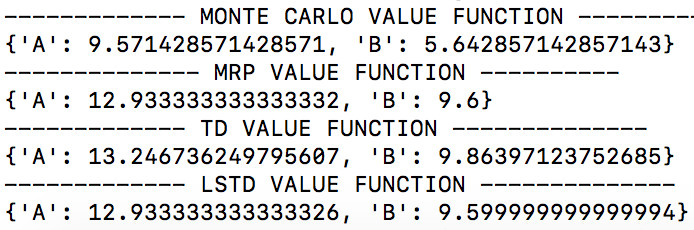
\includegraphics[width=0.5\linewidth]{various.png}
  \caption{Convergence of three control methods}
  \label{fig:optPol1}
\end{figure}


\section{TDC implementation and test}
We also implement the TDC algorithm and test with the random walk in random\_walk\_mrp.py. The implementation is below:

\begin{lstlisting}
class TDC:

    def __init__(
        self,
        feat_funcs: Sequence[Callable[[X],float]],
        alpha: float,
        beta: float
    ):
        self.feat_funcs = feat_funcs
        self.num_feats = len(feat_funcs)
        self.w = np.ones(self.num_feats)*0.2
        self.theta = np.zeros(self.num_feats)
        self.alpha = alpha
        self.beta = beta

    def featurize(self, s: X):
        return np.array([f(s) for f in self.feat_funcs])

    def update_weights(self,s:X,s_next:X,td:float, gamma:float):
        s_f = self.featurize(s)
        s_next_f = self.featurize(s_next)
        self.w = self.w + self.alpha*(td*s_f-gamma*s_next_f*np.dot(theta,s_f))
        self.theta = self.theta + self.beta*(td-np.dot(self.theta,s_f))*s_f

    def evaluate(self, s:X):
        return np.dot(self.w,self.featurize(s))

    def update_weights(self,s:X,s_next:X,reward:float, gamma:float, term:bool):
        s_f = self.featurize(s)
        s_next_f = self.featurize(s_next)
        td = reward+gamma*self.evaluate(s_next)*float(1-int(term)) - self.evaluate(s)
        self.w = self.w + self.alpha*(td*s_f-gamma*s_next_f*np.dot(self.theta,s_f)*float(1-int(term)))
        self.theta = self.theta + self.beta*(td-np.dot(self.theta,s_f))*s_f
        return self.alpha*(td*s_f-gamma*s_next_f*np.dot(self.theta,s_f))
     
    def learn_policy(self,mrp:MarkovRewardProcess[X], state_dist : Distribution[X], gamma:float, tolerance = 1e-5):
        count = 0
        while True:
            state = state_dist.sample()
            while(not(mrp.is_terminal(state))):
                state = state_dist.sample()
                next_state, reward = mrp.transition_reward(state).sample()
                diff = self.update_weights(state, next_state,reward,gamma, mrp.is_terminal(next_state))
                state = next_state
                count+=1
                if np.abs(diff) < tolerance:
                    return
\end{lstlisting}

We test the implementation with the random walk in 1D with 10 states and obtain very close to the correct value function:

 \begin{figure}[h]
  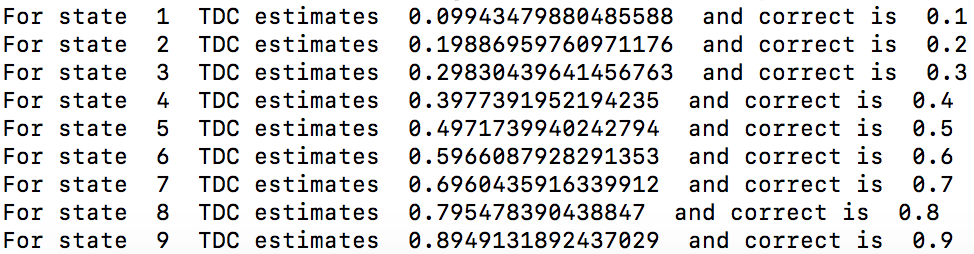
\includegraphics[width=0.75\linewidth]{mrp_results.png}
  \caption{Convergence of three control methods}
  \label{fig:optPol1}
\end{figure}

\end{document}
